\scanpage{74}
% archive sheet number: 75
Le système des inégalités \textcircled{17} (pour $m,n$ variables) et \uline{la conséquence (15)} semblent les inégalités les plus fortes possibles majorant \unsure{le|les} \inserted{\unsure{système|systèmes|fonction} des} $\rho_i(u+v)$ en fonction des $\rho_i(u)$, $\rho_i(v)$. Notons qu'on pourrait déduire \deleted{\unsure{de la même façon}} \inserted{directement} l'inégalité \uline{(15)} à partir de l'inégalité \uline{(12)} qu'elle \uline{généralise}, \uline{pour cela signalons} la \deleted{\unsure{prop}}

\uline{Prop. 4} Si $u\in L_0(E,F)$, \deleted{\unsure{et}} $n$ est un entier $>0$, on a

\[
\deleted{\unsure{d|\det}}\prod_1^n(1+\rho_i(u))=\operatorname{Sup}_{\substack{v_n\in L(F,E)\\\lVert v_n\rVert\leq1\\\operatorname{rang}v_n\leq n}}\det(1+v_nu)\tag*{(18)}
\]

Cette \deleted{démonstration} \inserted{formule} se démontre comme (17), \deleted{\unsure{on peut même}} \inserted{\deleted{\unsure{par}} le} raisonnement est \deleted{m\unsure{algré} \unsure{un} peu \unsure{simple}} \inserted{laissé au lecteur}

\figure{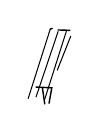
\begin{tikzpicture}[x=1mm,y=1mm,line cap=round]
\draw[line width=.13mm] (0,0)--(2.8,8.8) (1.0,.2)--(3.8,8.5) (2.1,-.1)--(4.9,8.7) (3.7,3.6)--(5.4,7.9);
\draw[line width=.18mm] (2.8,8.8)--(3.05,8.9) (3.8,8.7)--(5.3,8.65) (1.0,1.45)--(3.0,1.35)--(2.65,-.6) (1.8,1.4)--(2.1,-.7);
\end{tikzpicture}}
